%%
%% THESIS/DISSERTATION TEMPLATE FOR THE UNIVERSITY OF ALABAMA.
%%
%% This example is written by Paul Kilgo. It highlights all the (few) features
%% of uathesis.cls
%% Modified by Yuanyuan Song(2014) for the requirements of Ph.D thesis.

%% Use one of the following if writing a thesis/dissertation.
% \documentclass[thesis]{uathesis}
\documentclass[dissertation]{uathesis}

%% Basic packages you'll probably want to use.
\usepackage{graphicx}                 %% For using \includegraphics{}
\usepackage{cite}                     %% For sorting/collapsing citations.
\usepackage{color}                    %% For colors used in listings.
\usepackage{listings}                 %% Code listings (for engineers)
\usepackage{lipsum}
\usepackage[section]{placeins}
\usepackage{calc}
\usepackage{amsmath,array}
\usepackage{epstopdf}
\usepackage{morefloats}
\usepackage{subfig}
\usepackage{graphicx}
\usepackage[countmax]{subfloat}
%\usepackage[]{mcode}                 %% For including programming code
\usepackage{setspace}
%\usepackage{breqn}
%% Includes
%\input{inc/glossary.tex} %nomenclature
% TODO: If you have any special commands defined, include them here.

%%%%%%%%%%%%%%%%%%%%%%%%%%%New commands%%%%%%%%%%%%%%%%%%%%%%%%
\newcommand\Real{\mbox{Re}} % cf plain TeX's \Re and Reynolds number
\newcommand\Imag{\mbox{Im}} % cf plain TeX's \Im
\newcommand\Rey{\mbox{\textit{Re}}}  % Reynolds number
\newcommand\Ma{\mbox{\textit{Ma}}}  % Marangoni number
\newcommand\C{\mbox{\textit{C}}}  % Surfactant concentration
\newcommand\G{\mbox{\textit{G}}}
%\newcommand\A21{\mbox{\textit{\left[A\right]^2_1}}} % For the example of [A]^2_1
\newcommand\Ca{\mbox{\textit{Ca}}}  % Modified Capillary number
\newcommand\Or{\mbox{\textit{O}}}
\newcommand\slsA{\mathsfbi{A}} % for sans serif bold-sloping Q
\newcommand\etal{\mbox{\textit{et al.}}}
\newcommand\eps{\epsilon}
\newcommand{\pa}[2]{\frac{\partial #1}{\partial #2}}
\newcommand{\de}[2]{\frac{\mathrm{d} #1}{\mathrm{d} #2}}
\newcommand\Rsm{R_{sm}}
\newcommand\Rmg{R_{mg}}
\newcommand\Rw{R_{ws}}
\newcommand\Rwi{\overline{\Rw}}
\newcommand\Rsmi{\overline{\Rsm}}
\newcommand\Rmgi{\overline{\Rmg}}
\newcommand\Rj{{R_{j}}}
\newcommand\Rjz{{R_{j}}_z}
\newcommand\Rjzz{{R_{j}}_{zz}}
\newcommand\Rjzs{{R^\ast_{j}}_{z^\ast}}
\newcommand\Rjzzs{{R^\ast_{j}}_{z^\ast z^\ast}}
\newcommand\Rwz{{R_{ws}}_z}
\newcommand\Rsmz{{R_{sm}}_z}
\newcommand\Rmgz{{R_{mg}}_z}
\newcommand\Rwzz{{R_{ws}}_{zz}}
\newcommand\Rsmzz{{R_{sm}}_{zz}}
\newcommand\Rmgzz{{R_{mg}}_{zz}}
\newcommand\Rwt{{R_{ws}}_t}
\newcommand\Rsmt{{R_{sm}}_t}
\newcommand\Rmgt{{R_{mg}}_t}
\newcommand\ez{\eta_z}
\newcommand\az{\alpha_z}
\newcommand\bz{\beta_z}
\newcommand\gz{\mbox{\textit{G}}_z}
\newcommand\ezz{\eta_{zz}}
\newcommand\azz{\alpha_{zz}}
\newcommand\bzz{\beta_{zz}}
\newcommand\gzz{\mbox{\textit{G}}_{zz}}
\newcommand\ezzz{\eta_{zzz}}
\newcommand\azzz{\alpha_{zzz}}
\newcommand\bzzz{\beta_{zzz}}
\newcommand\gzzz{\mbox{\textit{G}}_{zzz}}
\newcommand\ezzzz{\eta_{zzz}}
\newcommand\azzzz{\alpha_{zzzz}}
\newcommand\bzzzz{\beta_{zzzz}}
\newcommand\gzzzz{\mbox{\textit{G}}_{zzzz}}
\newcommand\et{\eta_t}
\newcommand\at{\alpha_t}
\newcommand\bt{\beta_t}
\newcommand\gt{\mbox{\textit{G}}_t}
\newcommand\Rmgif{\Rmgi^4}
\newcommand\Rmgit{\Rmgi^2}
\newcommand\Rsmif{\Rmgi^4}
\newcommand\Rsmit{\Rsmi^2}


%%%%%%%%%%%%%%%%%%%%%%%%%%%%%%%%%%%%%%%%%%%%%%%%%%%%%%%%%%%%%%%%%


%% Required parameters (these default to undefined)
\author{Sheik Ahmed Ullah}       %% Your name!
\adviser{Shan Zhao}      %% Your adviser/committee chair!

%% The people on your committee.
%% Use \and to break them up between lines.
\committee{
  DAVID HALPERN \and
  BRENDAN AMES \and
  MUHAMMAD A. R. SHARIF \and
  MOJDEH RASOULZADEH
}

%% Note the use of \and to create line breaks and the
%% inverted pyramid style requested by the graduate school.

\title{A new ADI method for the Poisson-Boltzmann equation with a two-component regularization}

\degree{Doctor of Philosophy}   %% Change to suit your degree.
\department{Mathematics}        %% Change to suit your department.

%% These are body text paragraphs to be placed in the front matter.
\abstract{
The Poisson Boltzmann equation (PBE) is a well-established implicit solvent continuum model for the electrostatic analysis of solvated biomolecules. The solution for the nonlinear PBE is still a challenge due to its strong singularity by the source terms, dielectrically distinct regions, and exponential nonlinear terms. In this dissertation, a new alternating direction implicit method (ADI) is proposed for solving the nonlinear PBE using a two-component regularization. This scheme inherits all the advantages of the two-component regularization and the time-dependent PBE with ADI method while possess a novel approach to combine them. A modified version of the one-dimensional ghost fluid method (GFM) has been introduced to incorporate the nonzero jump condition into a new ADI method to propose GFM-ADI method. It produced better results in terms of  spatial accuracy and stability compared to the previous ADI method and simpler to implement by circumventing the work necessary to apply the MIB method with the regularization for a 3D problem. Moreover, the stability of the GFM-ADI method has been significantly improved in comparing with the non-regularized ADI method, so that stable protein simulations can be carried out with a pretty large time step size. Two locally one-dimensional (LOD) methods have also been developed for the time-dependent regularized PBE, which are unconditionally stable.  
%To continue the  search for more stable methods this modified GFM method and Locally One Dimensional (LOD) method has been combined similarly with Implicit Euler method and Crank-Nicolson method two propose GFM-LODCN and GFM-ODIE method. 
%{\color{red}Though this scheme can use larger time increments than the previous ADI method, it still blows up for large time increments. Later to address this issue with the stability, Locally One Dimensional (LOD) method has been used to replace the ADI method as the operator splitting part.} 
Finally, for numerical validation, we have evaluated the solvation free energy for a collection of 24 proteins with various sizes and the salt effect on the protein-protein binding energy of the complex 1beb.
}

\dedication{
To my loving parents and all the teachers in my life who inspired, helped and cared for me to pursue my interests in mathematics.  
}

\acknowledgments{
I wish to express my most sincere gratitude and appreciation to Professor Shan Zhao for his guidance, patience and encouragement. Without his help it would have been difficult for me to be focused to the right direction with all the patience and perseverance necessary before scholarly success. He has always been by my side as a local guardian and it meant a lot to me.  His funding from the NSF grant DMS-1812930 titled "{\it A regularized Poisson Boltzmann model for fast computation of the ensemble average polar solvation energy}" was also a great support for the last part of my Ph. D. program. 

I would also like to express my gratitude toward my committee members for their time and support: the external member from the Department of Aerospace Engineering and Mechanics at the University of Alabama, Dr. Muhammad Ali Rob Sharif and the local members from the Department of Mathematics at the University of Alabama, Dr. Brendan Ames, Dr. Mojdeh Rasoulzadeh and Professor David Halpern. I want to specially thank Professor Halpern for his help and guidance to get my access to the High Performance Computing facility from UAHPC and introducing me to the Summer School at the MSRI, UC Berkeley. I wish to express my indebtedness to Professor David Cruz-Uribe for his continuous support to arrange travel funds from the Graduate School, and the College of Arts and Sciences. 

I want to take this occasion to thank Dr. Weihua Geng from the Southern Methodists University and Professor Emil Alexov form the Clemson University for their help and support for my research projects on different occasions. Besides Professor Zhao, Dr. Geng is the second most important person who helped and guided me a lot to explore different areas on my research topic. 

I also want to recognize Dr. Khanh Dinh, David Neal, Dr. Xuan He, Dr. Timothy Homan and Summer Atkins for their friendship. Dr. Tania Hazra, Arum lee, Siwen Wang and Hongsong Feng were more than just group mates and always helpful. My former  roommate and a graduate student in the Department of Mechanical Engineering at UA, Md Abu Horaira Banna helped me to start using UAHPC which was an important skill to complete a major portion of the Numerical Validations for the proposed methods in this dissertation. 

Finally I want to thank my family for supporting me mentally through this program. My parents were always there to encourage and support my early mathematics education. I am really grateful for all the emotional support I got from my wife Elizabeth Brezovich and a lot of encouragement from her father Professor Ivan Brezovich.



}

%% Optional parameters. The default usage is shown.
\university{The University of Alabama}
\school{Graduate School}
\gradyear{2019}
\place{Tuscaloosa, Alabama}

\begin{document}


%% Makes the title, abstract, dedication, table of contents, etc.
%% Must be before \begin{body}
\makefrontmatter

%% BODY PORTION
%% The bulk of your thesis.
%% Begin your \chapter's here.

\begin{body}

%% Body chapters.
%---------------------------- Chapter 1 ----------------------------------------
\chapter{INTRODUCTION}
\label{chap: introduction}
Solvated biomolecules and their electrostatic interaction with the surrounding solvent are critical to the studies of various important biological processes such as protein-drug binding site analysis, DNA recognition, protein folding and protein ligand bonding. In the past few decades with the development of numerical methods and computational powers, the electrostatic analysis of functions and dynamics of bimolecular solvation has become more practical and effective. However, imitating these interactions are still computationally expensive with biological significance. Here we are considering the Poisson-Boltzmann Equation (PBE)  to describe the electrostatic potential generated by a low dielectric medium inside a protein molecule with embedded atomic charges solvated in a high dielectric medium with dissolved ions. The analytical solution of PBE is only available for some simple geometry such as a sphere or a cylinder. Efficiency and accuracy are still critical issues in numerical solution of the PBE for biophysical models with complex geometry, especially for macromolecules  containing tens of thousands to millions of atoms. 

 In our mathematical model for the electrostatic analysis, PBE is a nonlinear elliptic equation on multiple domains with discontinuous dielectric coefficients separated  by the solute-solvent interface or molecular surface. The difficulties with solving PBE arises from nonlinearity, discontinuous dielectric coefficients, non-smoothness of the solution and singularities in the source term due to the atomic charges. Effects of nonlinearity becomes significant with strong ionic presence~\cite{Wilson2016}. 


For the nonlinearity, two different approaches have been developed in the literature. The usual approach is to discretize the nonlinear PBE into an algebraic system using finite difference or finite element methods and then solve it by a nonlinear algebraic system such as nonlinear relaxation method \cite{Im1998}, \cite{Rocchia2001}, nonlinear conjugate gradient method~\cite{Luty1992} or inexact Newton method \cite{Holst1995}. The other approach has been introduced recently based on the  pseudo-transient continuation idea \cite{Shestakov2002,Sayyed-Ahmad2004,Zhao2011}. This approach converts the time independent nonlinear PBE into a time dependent form by introducing a pseudo-time derivative. The solution to the original boundary problem is then retrieved from the steady state solution of the time dependent PBE. The main advantage of introducing pseudo-time derivative is to be able to split time dependent PBE into linear and nonlinear subsystems to circumvent the blow up and overflow problem due to the exponentially large term involving the hyperbolic sine function. 

In pseudo-time methods, the time dependent PBE has to be solved until steady state. To maintain the efficiency, a large time increment for  $\Delta t$ is required. This is why the existing pseudo-time methods usually adopted an implicit scheme in time stepping. Moreover, to convert the three dimensional(3D) PBE into a set of multiple independent one-dimensional(1D) systems, the alternating direction implicit (ADI) methods in \cite{Geng2013_tree,Geng2013_Fully}, the locally one dimensional (LOD) method in \cite{Wilson2016} have been introduced in the literature. Especially in \cite{Geng2013_Fully} the Douglas-Rachford ADI scheme has been used to split the linear subsystem with the 3D laplacian operator into three sub-systems with one dimensional 2nd order derivatives. Altogether this method has first order accuracy in time but a quite severe stability condition. Later in \cite{Wilson2016} the LOD method was introduced as an unconditionally stable method with reduced accuracy compared to ADI methods in \cite{Geng2013_Fully}. Even though 1D subsystems produced by these ADI and LOD methods are tridiagonal and can be efficiently solved by using the Thomas Algorithm \cite{FD_PDE}, they lack the treatment of the jump conditions at the interface which reduces the spatial accuracy near the interface. Also the numerical error for these pseudo-transient methods has been observed often to be dominated by the the singularity at the center of the atoms.

Besides strong nonlinearity, the numerical treatment of charge singularity is another challenge for the PBE. At atom centers, both the charge source and the potential solution blow up, and the conventional discretization is doomed to be inaccurate. This motivated many authors to develop different regularization methods in \cite{Cai2009,Chen2007, Geng2007,Holst2010,XIE2014,Zhou_1996,Geng2017a} to reduce the loss of accuracy due to the singularity. In these methods, the potential function is decomposed into a singular component plus one or two other components to break down the PBE into a system of partial differential equations (PDEs) containing a Poisson equation with the singular term plus other equations. Thus the singular component can be handled separately using the analytical solution for the Poisson equation in terms of Coulomb potentials or Green's functions. So far these type of regularization methods have never been used with the ADI or LOD type pseudo-transient methods. 

The dielectric interface is also crucial in numerical discretization of the PBE as it defines the boundary for the solute and solvent regions. Across a geometrically complex dielectric interface, or molecular surface, the potential solution is continuous, but its normal derivative is discontinuous. For the un-regularized PBE, the standard finite difference method is still convergent but degenerates to first order convergence in space. However, the situation becomes worse for regularized PBE proposed by Luo \cite{Cai2009}, because now both the potential and its flux is discontinuous across the interface for the regularized solution. The standard finite difference solution will diverge in this case, if no interface treatment is imposed. For this reason, the regularized PBE is usually solved by some special interface schemes, such as the matched interface and boundary (MIB) method \cite{Geng2007,Chen2011,Yu2007,ZHAO2004,ZHOU2006,ZHOU2006_high,YU2007_3D}. We note that regularization methods have been applied with the finite element type pseudo transient methods in \cite{DENG2018}, in which the interface jump conditions can be built in the variational formulations. However, these methods are usually inefficient for the pseudo time approach by solving a non-symmetric linear system iteratively at each time step. 

In an attempt to maintain the efficiency and stability of the ADI methods while restoring the accuracy to the second order near the interface, several interface schemes have been developed for solving the diffusion equation in \cite{Li1999,Liu2013}. Then as a continuation of this approach recently matched ADI (mADI) method was developed in \cite{Zhao2015} and \cite{Li2017} to combine the MIB method (for interface treatment) with ADI. But these ADI methods were mainly focused on the parabolic equations and have never been applied to the PBE. In fact, the mADI \cite{Zhao2015} could become cumbersome in treating a complicated interface, like the molecular surface in protein studies. 

In this dissertation, our goal was to develop a new approach to solve the PBE combining the regularization, the pseudo-transient continuation and the interface treatment so that both nonlinearity and singularity are properly treated. For the regularization we have chosen  the two component regularization developed in \cite{Geng2017a} which is the simplest and most accurate regularization method. But it changes the jump condition to be non zero which introduces the necessity of interface treatments. Otherwise the standard central finite difference becomes divergent. Then motivated by the mADI method we have generalised the Ghost Fluid Method (GFM) developed in \cite{Fedkiw1999} as the interface treatment for the present study. Compared to mADI, GFM is simpler to apply in a pseudo-continuation approach. Altogether GFM-ADI method improved the accuracy and efficiency of the ADI method to solve the nonlinear PBE. Generally it is more robust than the ADI method but still has a time stability constraint when the time step size is too huge. Then to continue the search of a more stable method for our regularized pseudo continuation approach we replaced the ADI scheme by the LOD formulation to propose GFM-LODCN and GFM-LODIE methods. These two methods combine LOD  with Crank-Nicolson (CN) and Implicit Euler (IE) to discretize the pseudo time derivative. All of the three methods produced more accurate and efficient results  than their predecessors. Empirically GFM-LODIE has found to be most robust while GFM-ADI to be most accurate. 
%%%%%%%%%%%%%%%%%%%%%%%%%%%%%%%%%%%%%%%%%%%%%%%%%%%%%%%%%%%%%%%%%%%%%%%%%%%%%%%%%%%%%%%%%%%%%
\section{Outline of this dissertation}
There are six main parts in this dissertation. The first part discusses the protein data file preparations necessary for the numerical algorithm developed to calculate the electrostatic potential and the solvation energy by the PBE. The second part introduces the Poisson-Boltzmann model and discusses the ADI method \cite{Geng2013_Fully} to give an analytical background of the previous ADI methods, molecular surfaces and coding packages. The third part discusses the two component regularization and introduces three pseudo transient methods GFM-ADI, GFM-LODCN and GFM-LODIE.  The fourth part introduces a new GFM method to incorporate with the proposed pseudo transient methods. The last part validates the proposed method for a benchmark problem and examines the application of the newly proposed methods to the PBE model for the real proteins. Below is a breakdown of the following chapters in greater detail:  
  

{\bf Chapter \ref{chap: protein_data}} starts with a description of the Protein Data Bank and its different file formats. A detail description of {\it .pdb} file is included with the process to convert them to get the {\it .pqr} file. The types of inputs like the $x,y$ and $z$ coordinates, the Van der Walls radius and the charges for the numerical algorithms are discussed in detail. 

{\bf Chapter \ref{chap: PBE}} reviews the PB model with the Poisson-Boltzmann Equation which will be the problem at the center of the discussion in the rest of the dissertation. Different type of Molecular surfaces are reviewed to explain our choice of SES surface to be generated by the MSMS software. A detail description of the previous ADI method \cite{Geng2013_Fully} has been incorporated. At the end of the chapter the development of the software package REG-GFM-MSMS from ADI-MSMS are described. 

{\bf Chapter \ref{chap:opt_split}} reviews the two-component regularization and its incorporation with the pseudo-transient approaches. Three types of operator splitting methods are proposed in this chapter to the solve the PBE. An analytical background of the calculation of the solvation energy from the solution of the PBE are discussed.

{\bf Chapter \ref{chap:new_GFM}} introduces a modified version of the Ghost Fluid Method (GFM) and its detailed derivation. It also covers a background on other GFM methods.

{\bf Chapter \ref{chap:num_vald}} examines the numerical validation for the proposed three methods in chapter \ref{chap:opt_split} for the krikwood sphere problem and other biological problems. For the benchmark problem  several tests are performed to test the stability, the spatial convergence and the temporal convergence. Similar tests are performed to calculate the solvation energy for a collection of 24 proteins. To calculate other types of biological feature of proteins, the binding energy of HIV viral replication is performed. As the last test the salt effects on the binding energy of several proteins is calculated and compared with available experimental data.    

{\bf Chapter \ref{chap: conclusions}} finally summarizes the findings made in this dissertation and proposes some opportunities for future work.  


% --------------------------- Chapter 2 ----------------------------------------
\chapter{\MakeUppercase{Governing equations and boundary conditions for a bilayer coating a compliant tube}}\label{chap: Governing_Eqn_boundary_conditions_dim}
%%%%%%%%%%%%%%%%%%%nomenclatures%%%%%%%%%%%%%%%%%%%%%%%%
\nom{$g$}{the wall damping coefficient}
\nom{$k_c$}{the critical wavenumber where infinite growth rate occurs}
\nom{$\Ma$}{a measure of the ability of surfactant to lower the surface tension at the mucus-gas interface}
\nom{$Pe$}{\textit{P$\acute{e}$clet number}}
%% If you are using winedt instead of Kile or other compiler, in order to have nomenclature work, you will need to type in 'makeindex test123.nlo -s nomencl.ist -o test123.nls' into the command window(change test 123 to the name of your main file).
%\nom{$\Rey$}{Reynolds number}
%\nom{$r^\ast$}{the radial axis}
%\nom{$\displaystyle{s=\frac{{\sigma_{mg}}_0}{\sigma_{sm}}}$}{the surface tension ratio of the base state mucus-gas surface tension to the serous-mucus surface tension}
%\nom{$T_{\ell}$}{longitudinal wall tension to surface tension}
%\nom{$T_0$}{initial circumferential tension of the tube wall to the surface tension}
%\nom{$h_0$}{the initial thickness of the tube}
%\nom{$z^\ast$}{the axial axis}
%%%%%%%%%Greek%%%%%%%%%%
%\nom{$\gamma_w$}{the Poisson ratio}
%\nom{$\displaystyle{\gamma=\frac{\mu_m}{\mu_s}}$}{the viscosity ratio of the mucus layer to the serous layer}
%\nom{$\Gamma$}{tube wall surface tension forces to elastic forces}
%\nom{$\eps=\eps_s+\eps_m$}{the thickness of the bilayer to the tube radius}
%\nom{$\displaystyle{\lambda=\frac{\epsilon_s}{\eps}}$}{the thickness ratio of serous layer to the bilayer}
%\nom{$\mu_{i}$}{viscosity of the liquid layer, $i=$\textit{serous, mucus}}
%\nom{$\rho_w$}{the wall density}
%\nom{$\phi$}{the tube wall damping parameter}
%\nom{$E$}{the sensitivity of the surface tension to the surfactant concentration}
%\nom{$Pe$}{\textit{P$\acute{e}$clet number}}
%%%%%%%%%%%%%%%%%%%%%%%%%%%%%%%%%%%%%%%%%%%%%%%%%%%%%%%%%%%%%%%%%%%%%
%%%%%%%%%%%%%%%%%%Problem Description%%%%%%%%%%%%%%%%%%%%%%%%%%%%%%%%%
$g$, $k_c$, $\Ma$, and $Pe$
\begin{figure}[h]
\begin{center}
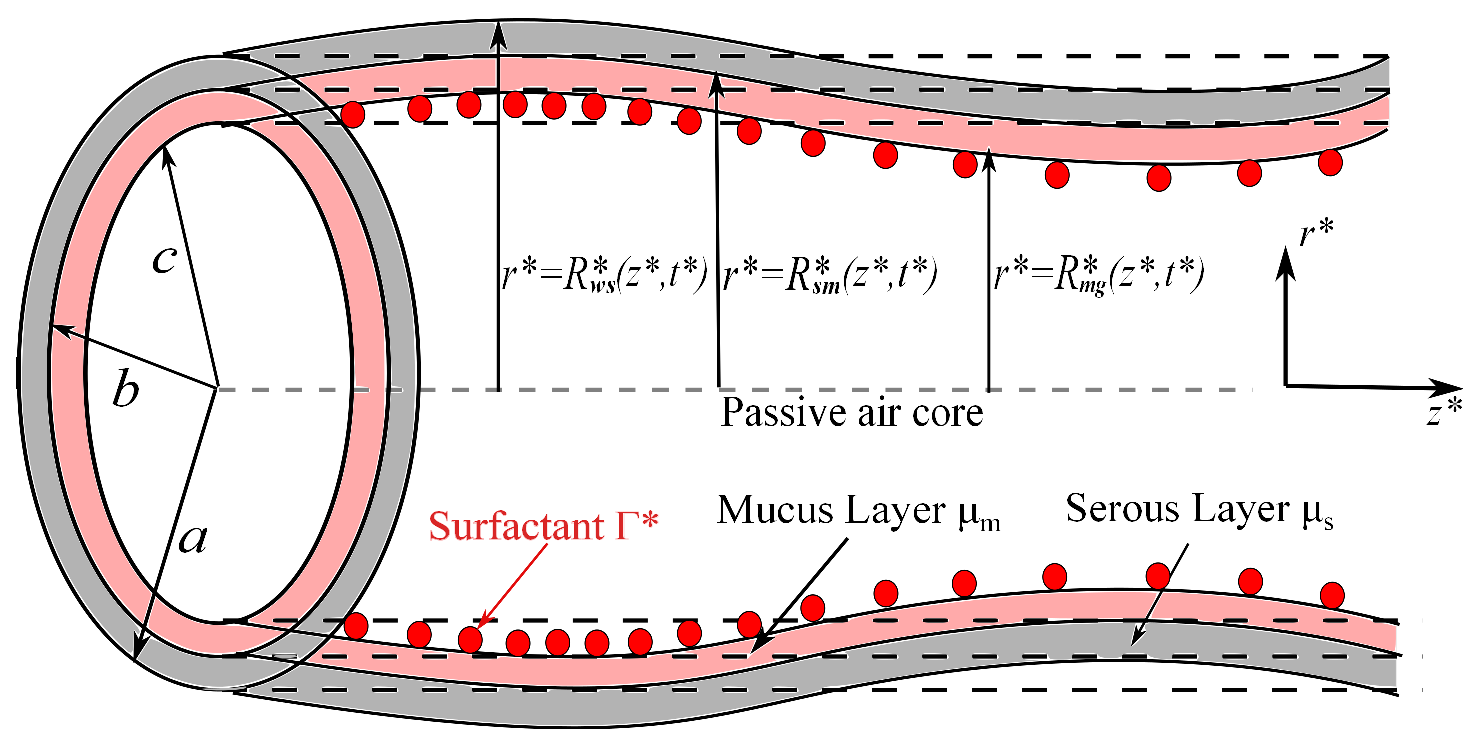
\includegraphics[width=0.98\textwidth]{geometry_full.eps}
\end{center}
\caption{A liquid bilayer coating a compliant cylindrical tube with an insoluble surfactant monolayer present at the \textit{gas-mucus} interface.}
\label{fig:geometry}
\end{figure}
\lipsum 
\chapter{THEORY AND ALGORITHM}
\label{chap: theory}
\input{theory}


%% -----------------------------Chapter 7 ---------------------------------------
\chapter{CONCLUSIONS}
\label{chap: conclusions}
The pseudo-transient methods and regularization methods are popular methods to solve nonlinear PBE. Even though these two types were successful in circumventing different challenges to solve PBE, each one of them was lacking the advantages of the other one. When we tried to combine them we faced a new challenge due to  the new jump conditions being nonzero. This forced us to find a way to apply interface treatments. The MIB method \cite{Geng2007,Chen2011,Yu2007,ZHAO2004,ZHOU2006,ZHOU2006_high,YU2007_3D} was a great choice for this type of interface treatments but it would have ruined the tridiagonal structure of the finite difference operator matrix of the 1D equations like (\ref{GFM-ADI}) (\ref{GFM-ADI2}) and (\ref{GFM-ADI3}) in all of our proposed methods. Having tridiagonal structure for these three equations are very important since we have to solve all three of them at each time step. So for small time step size, it would take unreasonably long time for the whole system to reach the equilibrium state to produce the solution.   

So we considered the GFM method \cite{Liu2000} for $L=1$ which uses a three point stencil keeping the tridiagonal structure for the 1D equations in our proposed methods. But the original GFM method requires the jump conditions to be in axial directions while the regularized PBE has its jump condition in the normal direction. It motivated us to modify the original GFM  method to able to use the normal direction jump condition by considering approximate jump conditions like (\ref{eq:m-gfm1}) and (\ref{eq:m-gfm2}). 

In comparison with the existing pseudo-transient approaches the GFM-ADI proposed in this dissertation is much more stable than ADI in \cite{Geng2013_Fully}. This makes GFM-ADI a very practical method, while the ADI method is impractical by requiring too small time step size. In some sense, the GFM-ADI method is even better than LOD methods in \cite{Wilson2016}. Although LOD methods are unconditionally stable, energies are inaccurate for large time steps. GFM-LODCN and GFMLOD are also producing more accurate results than its predecessor the LOD methods in \cite{Wilson2016} leaving an option for the cases when GFM-ADI fails to converge. 

In future we have a plan to take the advantage of the simplicity of these proposed schemes to the other areas of molecular biophysics like the problem of computing the electrostatic field and forces for molecular dynamic simulations as in \cite{GENG_WEI2011}. 
 

%% ---------------------------- Reference ---------------------------------------
%% Suggestion: Jabref is a nice free software for references which is compatible with Goodschalor cite function.
\addcontentsline{toc}{chapter}{REFERENCES}
\renewcommand{\bibname}{REFERENCES}
\begin{singlespace}
\bibliography{bibl}
\bibliographystyle{abbrv}
\label{bib}
\end{singlespace}

%%%%%%%%%%%%%%%%%%APPENDIX%%%%%%%%%%%%%%%%%%%%%%
\addcontentsline{toc}{chapter}{APPENDIX}
\appendix

\lipsum








\end{body}
\end{document}
